\RCS$Revision: $
\RCS$HeadURL: $
\RCS$Id: $



%The particle content of the minimal supersymmetric standard
%model~\cite{ref:SUSY2} can be summarized as follows. The superpartners
%to the gluons, quarks, and leptons are the gluinos $\PSg$, the
%light-flavour $\PSQ$, bottom $\PSQb$, and top $\PSQt$ squarks, and the
%sleptons $\PSl$, respectively. An extended Higgs sector comprising a
%quintet of scalar particle states is predicted. The higgsino and
%gaugino superpartners to the Higgs and electroweak gauge bosons are
%expected to mix to give six observable states: two charginos
%$\PSGcpm_{1,2}$ and four neutralinos $\PSGcz_{1,2,3,4}$.



%\begin{table}[tb!]
%  \topcaption{Lower bounds of \scalht bins [GeV] used in the control 
%    regions, and \alphat and \bdphi thresholds as a function of
%    \scalht. For monojet events, \bdphimod replaces \bdphi with 
%    identical thresholds.}  
%  \label{tab:thresholds}
%  \centering
%  \begin{tabular}{ lccccccccccc }
%    \hline
%    Variable & \multicolumn{11}{c}{\scalht [GeV]}                                           \\
%%    \cline{2-8}
%             & 200  & 250  & 300  & 350  & 400  & 500  & 600  & 750  & 900 & 1050 & $>$1200 \\
%    \hline                                                                         
%    \alphat  & 0.65 & 0.60 & 0.55 & 0.53 & 0.52 & 0.52 & 0.52 & 0.52 & --  & --   & --      \\
%    \bdphi   & 0.5  & 0.5  & 0.5  & 0.5  & 0.5  & 0.5  & 0.5  & 0.5  & 0.5 & 0.5  & 0.5 \B    \\
%    \hline
%  \end{tabular}
%\end{table}



%Figure~\ref{fig:alphat-bdphi} shows the \alphat and \bdphi
%distributions observed in data for events that satisfy all other
%signal region selection criteria plus $\scalht > 300\GeV$ and $\scalht
%> 800\GeV$, respectively. In the case of the \alphat distribution, the
%events that satisfy $\alphat < 0.55$ must only fulfill the baseline
%selection criteria defined in Table~\ref{tab:selections}, no \mht
%requirement is made, and the events are recorded with an unbiased set
%of trigger \scalht conditions.

%\begin{figure*}[tb!]
%  \begin{center}
%    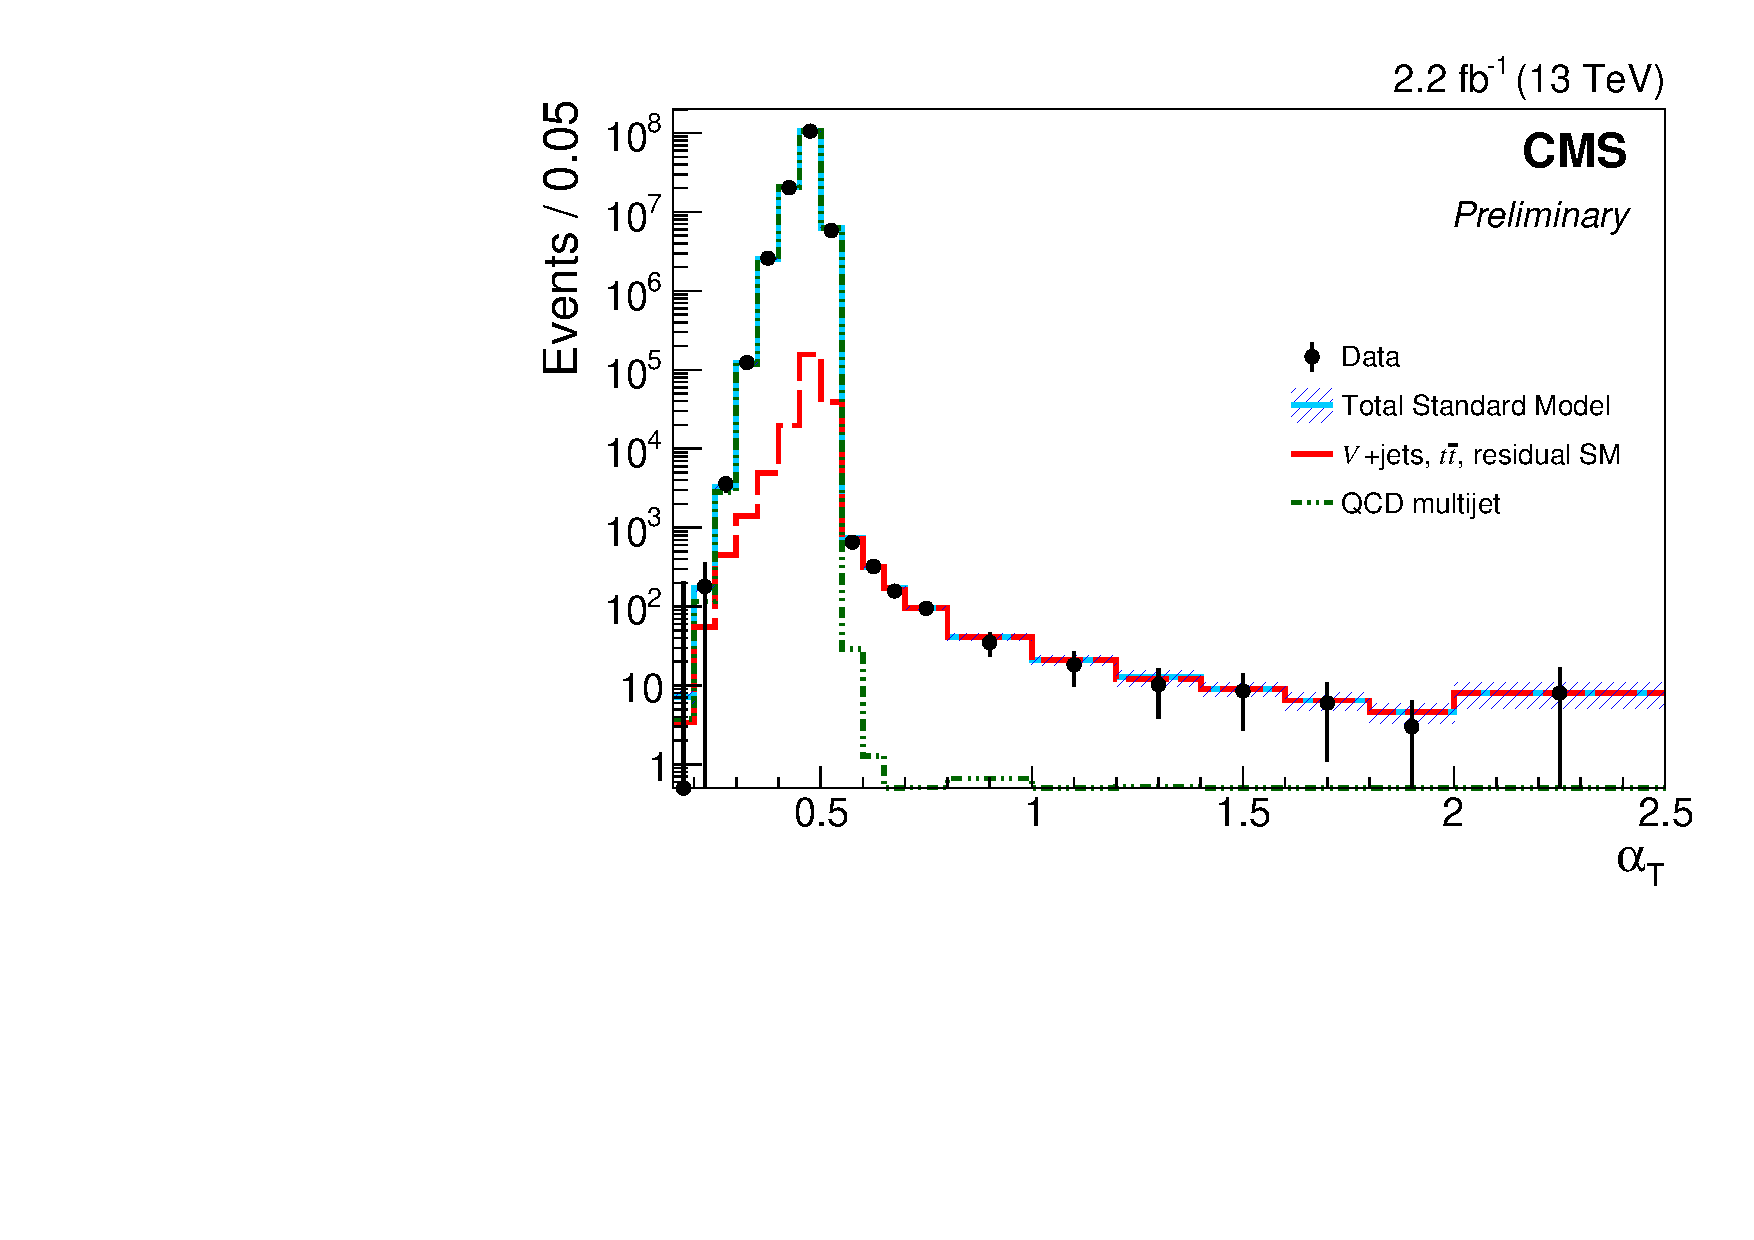
\includegraphics[width=0.49\textwidth]{alphaT_v4} \,
%    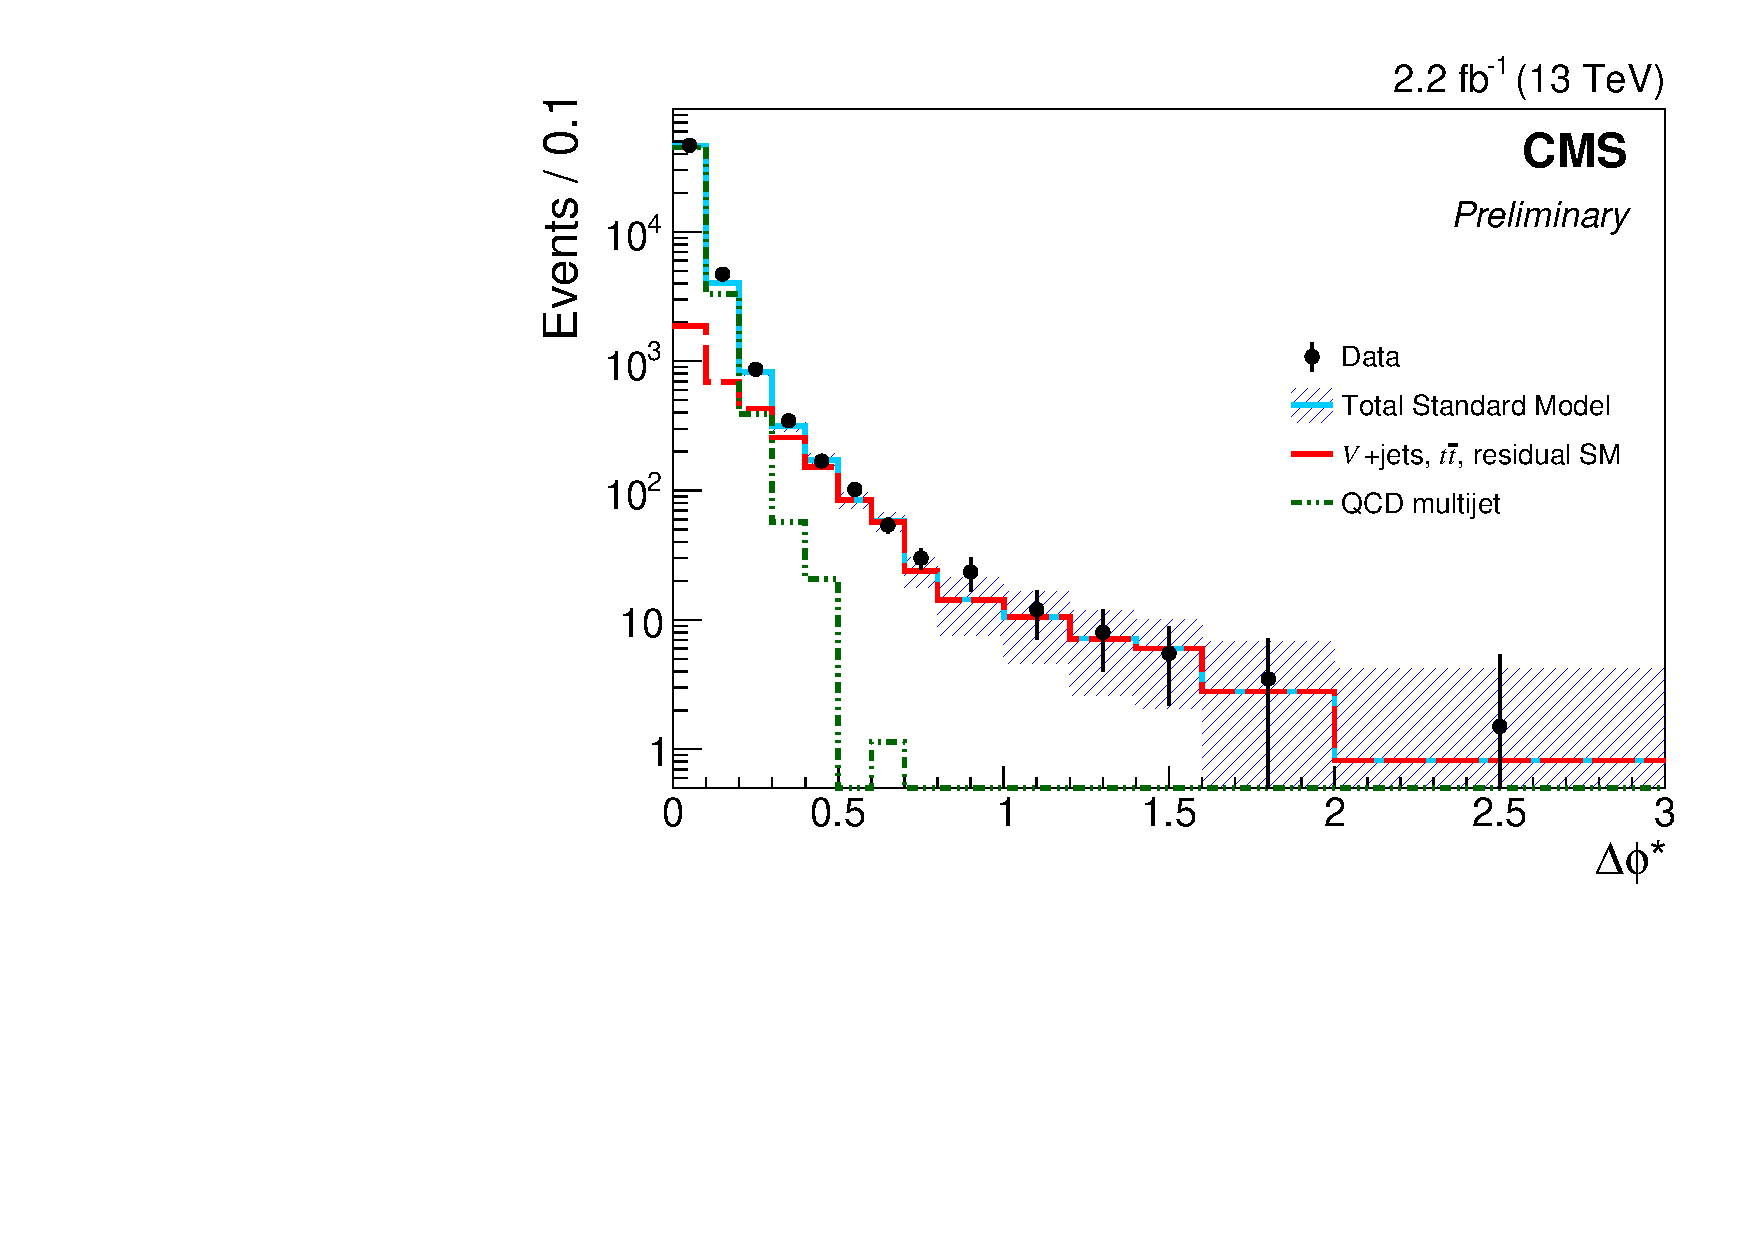
\includegraphics[width=0.49\textwidth]{bDPhi_v4} \\
%  \end{center}
%  \caption{(Left) The \alphat distribution observed in data for events
%    that are recorded with unbiased trigger conditions and satisfy the
%    baseline (full signal region) selection criteria for the region
%    $\alphat < 0.55$ ($\alphat > 0.55$). (Right) The \bdphi
%    distribution observed in data for events that satisfy the full
%    signal region selection criteria and $\scalht > 800\GeV$.  The
%    distributions for the QCD multijet backgrounds are determined from
%    simulation while all other SM backgrounds are estimated using a
%    $\mu$ + jets data control sample. %The uncertainties in the SM
%    %expectation are dominated by the statistical uncertainties 
%    %associated with the limited sample of simulated multijet events.
%    \label{fig:alphat-bdphi} 
%  }
%\end{figure*}



%\begin{table}[tb!]
%  \topcaption{Efficiency $\varepsilon_\textrm{trig}$ [\%] of the
%    signal triggers as a function of \scalht after applying the signal
%    region selection criteria, as determined from data. The first
%    (asymmetric) and second set of are statistical and systematic in
%    nature. 
%  } 
%%  \footnotesize
%  \centering
%  \begin{tabular}{lcccc} 
%    \hline
%    \scalht [GeV]                    & 200--400 & 400--600 & 600--900 & $>$900 \\
%    \hline
%    $\varepsilon_\textrm{trig}$ [\%] & $97.4^{+0.5}_{-0.6}{}^{+0.6}_{-0.6}$ 
%                                     & $97.9^{+0.8}_{-1.2}{}^{+1.0}_{-1.0}$ 
%                                     & $100.0^{+0.0}_{-1.8}{}^{+0.0}_{-0.6}$ 
%                                     & $100.0^{+0.0}_{-3.6}{}^{+0.0}_{-0.1}$ \B  \\
%    \hline
%  \end{tabular}
%  \label{tab:triggers}
%\end{table}

%Candidate signal events are recorded with a number of trigger
%conditions. Trigger logic requiring the presence of significant \mht
%and \ptmiss is used to record events containing one or more
%jets. Additional logic is used that simultaneously requires
%predetermined thresholds on \scalht and \alphat to be
%satisfied. Finally, a trigger condition based solely on \scalht is
%used to record candidate events for the region $\scalht >
%900\GeV$. The combined trigger strategy provides high efficiencies for
%all event categories of the the signal region, which are primarily
%dependent on \scalht, as summarized in Table~\ref{tab:triggers}.



%\begin{table}[!tb]
%  \topcaption{Variables used to categorize events for the signal and
%    control regions and the total number of bins. 
%%    The number in parentheses represent the maximum number of bins
%%    possible for each variable.   
%  }
%  \label{tab:catfinal}
%  \centering
%  \begin{tabular}{ llc }
%    \hline
%    Region    & Variables                                 & Bins     \\
%    \hline
%    Signal    & \njet, \scalht, \nb, \mht                 & 274      \\
%    \mj       & \njet, \scalht, \nb                       & 207      \\
%    \mmj      & \njet, \scalht                            & \ph{2}61 \\
%    Multijet  & \njet, \scalht                            & \ph{2}30 \\
%%    Signal   & \njet (7), \scalht (5), \nb (5), \mht (4) & 274      \\
%%    \mj      & \njet (7), \scalht (11), \nb (5)          & 207      \\
%%    \mmj     & \njet (7), \scalht (11)                   & \ph{2}61 \\
%%    Multijet & \njet (7), \scalht (5)                    & \ph{2}30 \\
%    \hline
%  \end{tabular}
%\end{table}



%\begin{table}[!tb]
%  \topcaption{Lower bound for the final open \scalht bin [GeV] used in
%    the search as a function of \njet and \nb. A dash (--) signifies a
%    category that is not used. The label {\it a} signifies the
%    asymmetric topology. 
%}
%  \label{tab:categorization}
%  \centering
%  \begin{tabular}{ lccc }
%    \hline
%    $\njet\, / \,\nb$ & 0         & 1         & ${\geq}2   \\
%    \hline
%    1                 & \ph{1}900 & \ph{1}600 & --        \\ 
%    ${\geq}2{\it a}    & \ph{1}900 & \ph{1}900 & \ph{1}400 \\ 
%    2                 & 1200      & 1200      & \ph{1}200 \\ % CHANGE TO 400!
%    3                 & 1200      & 1200      & \ph{1}600 \\ 
%    4                 & 1200      & 1200      & \ph{1}900 \\ 
%    5                 & 1200      & 1200      & \ph{1}900 \\ 
%    ${\geq}6           & 1200      & 1200      & \ph{1}900 \\ 
%    \hline
%  \end{tabular}
%\end{table}



%\subsection{Simplified binning scheme}
%\label{sec:aggregated}
%
%Data counts and SM background estimates are aslo provided for an
%alternate, simplified binning scheme in which events are organized
%into eight distinct topologies defined in terms of \njet and \nb, as
%summarized in Table~\ref{tab:aggrsr}. For each topology, event yields
%are integrated over the full \scalht range, $\scalht > 200\GeV$, and
%categorized according to the four bins in \mht defined above. This
%scheme leads to 32 bins that are exclusive, contiguous, and provide a
%complete coverage of the signal region. The SM background estimates
%are based on the same likelihood model used to determine the nominal
%result.
%
%\begin{table}[!tb]
%  \centering
%  \caption{The event topologies, defined in terms of
%    requirements on \njet and \nb, for the simplified binning
%    scheme. Events are further categorized according to four \mht bins
%    per topology.
%    \label{tab:aggrsr}
%  }
%  \begin{tabular}{lccc}
%    \hline
%    Topology     & \njet categories  & Low \nb & High \nb \\
%    \hline
%    Monojet-like & 1, ${\geq}2{\it a} & 0--1    & ${\geq}2  \\
%    Low \njet    & 2, 3              & 0       & ${\geq}1  \\
%    Medium \njet & 3, 4              & 0--1    & ${\geq}2  \\
%    High \njet   & 5, ${\geq}6        & 0--2    & ${\geq}3  \\
%    \hline
%  \end{tabular}
%\end{table}



%    QCD + EWK NLO corrections           & 0.5--5.4           & 2.2--14.3             \\
%    $N_\textrm{isr}$ (\ttbar)           & 0.8--1.1           & --                    \\
%    Signal trigger efficiency           & 0.0--3.1           & 0.0--2.0              \\
%    Muon trigger and selection          & 0.0--2.1           & 0.0--4.2              \\
%    Lepton vetoes                       & X--Y               & X--Y                  \\
%    Jet energy scale                    & 3.4--5.5           & 5.3--8.0              \\
%    b-quark tag efficiency              & 0.4--0.6           & 0.3--0.6              \\
%    b-quark mistag probability          & 0.1--1.4           & 0.2--1.8              \\



%A summary of the limits is provided in
%Table~\ref{tab:simplified-models-limits}.

%\newcommand{\ph}{\ensuremath{\phantom{1}}}
%\begin{table}[tb]
%  \topcaption{Summary of the mass limits obtained for the four 
%    classes of simplified models. The limits indicate the strongest
%    observed (expected) mass exclusions for the gluino or squarks, and
%    $\chiz_1$, and the quoted values have uncertainties of
%    $\pm$25\GeV.  
%  }
%  \label{tab:simplified-models-limits}
%  \centering
%  \footnotesize
%  \begin{tabular}{ llcc }
%    \hline
%    Production mode & Squark & \multicolumn{2}{c}{Strongest obs. (exp.) mass exclusion [GeV]}\T\B \\
%    \cline{3-4}                     
%                    &        & Gluino or squark\T\B & \chiz                                       \\
%    \hline                          
%    Gluino-mediated & Bottom & 1775 \ph(1850)       & 1175 \ph(1200)                              \\ 
%    Gluino-mediated & Top    & 1450 \ph(1600)       & \ph750 \ph\ph(800)                          \\ 
%    Direct          & Bottom & 1025 \ph\ph(975)     & \ph525 \ph\ph(500)                          \\ 
%    Direct\B        & Top    & \ph875 \ph\ph(925)   & \ph350 \ph\ph(350)                          \\
%    \hline
% \end{tabular}
%\end{table}



%\begin{table}[!tb]
%  \topcaption{Lower bound for the final open \scalht bin [GeV] used in
%    the search as a function of \njet and \nb. A dash (--) signifies a
%    category that is not used. The label {\it a} signifies the
%    asymmetric topology. 
%}
%  \label{tab:categorization}
%  \centering
%  \begin{tabular}{ lccccc }
%    \hline
%    $\njet\, / \,\nb$ & 0         & 1         & 2         & 3         & ${\geq}4$ \\
%    \hline
%    1                 & \ph{1}900 & \ph{1}900 & --        & --        & --        \\ 
%    ${\geq}2a$        & \ph{1}900 & \ph{1}900 & \ph{1}900 & \ph{1}600 & --        \\ 
%    2                 & 1200      & 1200      & \ph{1}900 & --        & --        \\ 
%    3                 & 1200      & 1200      & 1200      & \ph{1}900 & --        \\ 
%    4                 & 1200      & 1200      & 1200      & \ph{1}900 & --        \\ 
%    5                 & 1200      & 1200      & 1200      & \ph{1}900 & 400       \\ 
%    ${\geq}6$         & 1200      & 1200      & 1200      & 1200      & 400       \\ 
%    \hline
%  \end{tabular}
%\end{table}



%\begin{table}[!tb]
%  \centering
%  \caption{The event topologies, defined in terms of
%    requirements on \njet and \nb, for the simplified binning
%    scheme. Events are further categorized according to four \mht bins
%    per topology.
%    \label{tab:aggrsr}
%  }
%  \begin{tabular}{lccc}
%    \hline
%    Topology     & \njet categories    & Low \nb & High \nb  \\
%    \hline
%    Monojet-like & 1, ${\geq}2{\it a}$ & 0--1    & ${\geq}2$ \\
%    Low \njet    & 2, 3                & 0       & ${\geq}1$ \\
%    Medium \njet & 3, 4                & 0--1    & ${\geq}2$ \\
%    High \njet   & 5, ${\geq}6$        & 0--2    & ${\geq}3$ \\
%    \hline
%  \end{tabular}
%\end{table}



%\begin{table}[!tb]
%  \topcaption{Summary of the lower bound on \scalht [GeV] for the 
%    ({\it first, final open}) bins used in the search as a function of
%    \njet and \nb. A dash (--) signifies a category that is not
%    used. The label {\it a} signifies the asymmetric topology.
%  }
%  \label{tab:categorization}
%  \centering
%  \begin{tabular}{ lccccc }
%    \hline
%    $\njet\, / \,\nb$ & 0                & 1                & 2                & 3                & ${\geq}4    \\
%    \hline
%    1                 & (200, \ph{1}900) & (200, \ph{1}900) & --               & --               & --         \\ 
%    ${\geq}2{\it a}    & (200, \ph{1}900) & (200, \ph{1}900) & (200, \ph{1}900) & (200, \ph{1}600) & --         \\ 
%    2                 & (200, 1200)      & (200, 1200)      & (200, \ph{1}900) & --               & --         \\ 
%    3                 & (200, 1200)      & (200, 1200)      & (200, 1200)      & (200, \ph{1}900) & --         \\ 
%    4                 & (400, 1200)      & (400, 1200)      & (400, 1200)      & (400, \ph{1}900) & --         \\ 
%    5                 & (400, 1200)      & (400, 1200)      & (400, 1200)      & (400, \ph{1}900) & (400, 400) \\ 
%    ${\geq}6           & (400, 1200)      & (400, 1200)      & (400, 1200)      & (400, 1200)      & (400, 400) \\ 
%    \hline
%  \end{tabular}
%\end{table}



%\begin{table}[!tb]
%  \topcaption{Threshold values for the final \nb categories used in the 
%    search, as a function of \njet and the lower bounds of \scalht
%    bins [GeV]. A dash (--) signifies a (\njet, \scalht) category that
%    is not used. The label {\it a} signifies the asymmetric $\njet
%    \geq 2$ topology. The symbol ${\geq} indicates a final category
%    that covers a range of values \nb, bounded by the condition $\nb
%    \leq \njet$ unless the \njet category is also unbounded.
%  }
%  \label{tab:catttw}
%  \centering
%  \begin{tabular}{ lrrrrr }
%    \hline
%    $\njet\, / \,\scalht$ [GeV] & 200     & 400     & 600     & 900     & $>$1200 \\
%    \hline
%    1                           & 1       & 1       & 1       & ${\geq}0 & --      \\ 
%    ${\geq}2{\it a}              & ${\geq}3 & ${\geq}3 & ${\geq}3 & ${\geq}2 & --      \\ 
%    2                           & 2       & 2       & 2       & 2       & ${\geq}1 \\ 
%    3                           & 3       & 3       & 3       & 3       & ${\geq}2 \\ 
%    4                           & --      & ${\geq}3 & ${\geq}3 & ${\geq}3 & ${\geq}2 \\ 
%    5                           & --      & ${\geq}4 & ${\geq}3 & ${\geq}3 & ${\geq}2 \\ 
%    ${\geq}6                     & --      & ${\geq}4 & ${\geq}3 & ${\geq}3 & ${\geq}3 \\ 
%    \hline
%  \end{tabular}
%\end{table}



%\begin{table}[!tb]
%  \topcaption{}
%  \label{tab:catzinv}
%  \centering
%  \begin{tabular}{ lrrrrr }
%    \hline
%    $\njet\, / \,\scalht$ [GeV] & 200     & 400     & 600     & 900     & $>$1200 \\
%    \hline
%    1                           & 1       & 1       & 1       & ${\geq}0 & --      \\ 
%    ${\geq}2{\it a}              & ${\geq}2 & ${\geq}2 & ${\geq}1 & ${\geq}1 & --      \\ 
%    2                           & 2       & ${\geq}1 & ${\geq}1 & ${\geq}1 & ${\geq}1 \\ 
%    3                           & ${\geq}2 & ${\geq}2 & ${\geq}2 & ${\geq}1 & ${\geq}1 \\ 
%    4                           & --      & ${\geq}2 & ${\geq}2 & ${\geq}2 & ${\geq}1 \\ 
%    5                           & --      & ${\geq}2 & ${\geq}2 & ${\geq}2 & ${\geq}1 \\ 
%    ${\geq}6                     & --      & ${\geq}2 & ${\geq}2 & ${\geq}2 & ${\geq}1 \\ 
%    \hline
%  \end{tabular}
%\end{table}



%\begin{table}[!h]
%  \topcaption{}
%  \label{}
%  \small
%  \centering
%  \begin{tabular}{lllllll}
%    \hline
%njet & nb   & HT200  & HT400       & HT600            & HT900                 & HT1200                         \\
%    \hline                                                                                                     \\
%eq1j & eq0b & $>$200 & $>$400      & $>$600           & $>$900                & --                             \\
%eq1j & eq1b & $>$200 & $>$400      & $>$600           & --                    & --                             \\
%ge2a & eq0b & $>$200 & 200, $>$400 & 200, 400, $>$600 & 200, $>$900           & --                             \\
%ge2a & eq1b & $>$200 & 200, $>$400 & 200, 400, $>$600 & 200, $>$900           & --                             \\
%ge2a & eq2b & $>$200 & 200, $>$400 & 200, 400, $>$600 & 200, $>$900           & --                             \\
%ge2a & eq3b & $>$200 & 200, $>$400 & 200, 400, $>$600 & --                    & --                             \\
%eq2j & eq0b & $>$200 & 200, $>$400 & 200, 400, $>$600 & 200, 400, 600, $>$900 & 200, 400, 600, $>$900          \\
%eq2j & eq1b & $>$200 & 200, $>$400 & 200, 400, $>$600 & 200, 400, 600, $>$900 & 200, 400, 600, $>$900          \\
%eq2j & eq2b & $>$200 & 200, $>$400 & 200, 400, $>$600 & --                    & --                             \\
%eq3j & eq0b & $>$200 & 200, $>$400 & 200, 400, $>$600 & 200, 400, 600, $>$900 & 200, 400, 600, $>$900          \\
%eq3j & eq1b & $>$200 & 200, $>$400 & 200, 400, $>$600 & 200, 400, 600, $>$900 & 200, 400, 600, $>$900          \\
%eq3j & eq2b & $>$200 & 200, $>$400 & 200, 400, $>$600 & 200, 400, 600, $>$900 & 200, 400, 600, $>$900          \\
%eq3j & eq3b & $>$200 & 200, $>$400 & 200, 400, $>$600 & --                    & --                             \\
%eq4j & eq0b & --     & 200, $>$400 & 200, 400, $>$600 & 200, 400, 600, $>$900 & 200, 400, 600, $>$900          \\
%eq4j & eq1b & --     & 200, $>$400 & 200, 400, $>$600 & 200, 400, 600, $>$900 & 200, 400, 600, $>$900          \\
%eq4j & eq2b & --     & 200, $>$400 & 200, 400, $>$600 & 200, 400, 600, $>$900 & 200, 400, 600, $>$900          \\
%eq4j & eq3b & --     & 200, $>$400 & 200, 400, $>$600 & 200, 400, 600, $>$900 & --                             \\
%eq5j & eq0b & --     & 200, $>$400 & 200, 400, $>$600 & 200, 400, $>$600      & 200, 400, 600, $>$900          \\
%eq5j & eq1b & --     & 200, $>$400 & 200, 400, $>$600 & 200, 400, $>$600      & 200, 400, 600, $>$900          \\
%eq5j & eq2b & --     & 200, $>$400 & 200, 400, $>$600 & 200, 400, $>$600      & 200, 400, 600, $>$900          \\
%eq5j & eq3b & --     & 200, $>$400 & 200, 400, $>$600 & 200, 400, $>$600      & --                             \\
%eq5j & ge4b & --     & 200, $>$400 & --               & --                    & --                             \\
%ge6j & eq0b & --     & $>$200      & 200, $>$400      & 200, 400, $>$600      & 200, 400, 600, $>$900          \\
%ge6j & eq1b & --     & $>$200      & 200, $>$400      & 200, 400, $>$600      & 200, 400, 600, $>$900          \\
%ge6j & eq2b & --     & $>$200      & 200, $>$400      & 200, 400, $>$600      & 200, 400, 600, $>$900          \\
%ge6j & eq3b & --     & $>$200      & 200, $>$400      & 200, 400, $>$600      & 200, 400, 600, $>$900          \\
%ge6j & ge4b & --     & $>$200      & --               & --                    & --                             \\
%    \hline
%  \end{tabular}
%\end{table}
